\documentclass[8pt,dvipsnames]{beamer}

\usetheme[progressbar=frametitle]{metropolis}
% \useoutertheme{progress1}
% \usepackage{pgfpages}
% \setbeameroption{show notes} % after pgfpages to works properly
% \setbeameroption{show notes on second screen=right}

% \useoutertheme{miniframes}      % add header navigation bar
% \usecolortheme[dark]{solarized}

% Change block size
% https://github.com/matze/mtheme/issues/307#issuecomment-502212780
% map default block to old-block

% \let\oldblock\block
% \let\endoldblock\endblock
% \renewenvironment{block}[1]{\begin{oldblock}{#1}\vspace{0pt}}{\end{oldblock}} % change block by adding smallskip


% Font configuration
\usepackage{fontspec}
\usepackage{unicode-math}
% Math Fonts
\usepackage{amsmath}
\usepackage{amssymb}
% \usepackage[mathrm=sym]{unicode-math}
% \setmathfont{Fira Math}
% \setmathfont{Latin modern Math}

% my packages
\usepackage{bookmark}
\usepackage{tikz}
\usetikzlibrary{tikzmark,calc,decorations.pathreplacing}
\usepackage{pgfplots}
\usepackage{multicol}
\usepackage{kmath}
\usepackage[absolute,overlay]{textpos} % provide textblock \begin{textblock}{WIDTH}(XCOORDINATE,YCOORDINATE)
\usepackage{xfrac}
\usepackage{pifont} % provide cmark and xmark
\usepackage{adjustbox} % provide includegraphics with percentage
\usepackage{booktabs} % toprule

% \usepackage[texcoord,grid,gridunit=mm,gridcolor=black!30,subgridcolor=gray!20]{eso-pic}

% my colors
\definecolor{darkblue}{HTML}{154360}
\definecolor{bluegreen}{HTML}{228BE6}
\definecolor{mygreen}{RGB}{30,132,73}
\definecolor{myred}{RGB}{179,30,0}
\definecolor{myblue}{HTML}{228BE6}

% bibliography


% % my commands
% my definition blocks

% Clement Elvira's colors
% \newenvironment{mydefblock}[1]{
%     \setbeamercolor{block title}{fg=white,bg=darkblue}
%     \setbeamercolor{block body}{fg=black,bg=bluegreen!10}
%     \begin{block}{#1}}{\end{block}}

% Toogle filled blocks
% \newenvironment{filledalertblock}[1]{
%     \metroset{block=fill}
%     \begin{alertblock}{#1}}{\end{alertblock}}

\newenvironment{mydefblock}[1]{%
    \metroset{block=fill}
    \begin{alertblock}{#1}}%
    {\end{alertblock}}

\newenvironment<>{mysotablock}[1][]{%
    \setbeamercolor{postit}{fg=black,bg=bluegreen!10}
    \begin{beamercolorbox}[sep=.2em]{postit}#1}{\end{beamercolorbox}}

\newenvironment<>{mycontriblock}[1][]{%
  \setbeamercolor{postit}{fg=black,bg=mygreen!20}
  \begin{beamercolorbox}[sep=.2em]{postit}#1}{\end{beamercolorbox}}

\newcommand{\myThankTo}[1]{\textcolor{cyan}{(\faPeopleCarry~#1)}}

\newcommand{\rotate}[1]{\rotatebox[origin=c]{-120}{#1}}
\newcommand{\iconAOA}{\rotate{\faArrowsAltH}}
\newcommand{\iconDOA}{\faArrows*}
\newcommand{\iconAz}{\faArrowsAltH}
\newcommand{\iconEl}{\faArrowsAltV}
\newcommand{\iconAlert}{\faExclamationTriangle}

\newcommand{\pro}[1]{\textcolor{mygreen}{#1}}
\newcommand{\con}[1]{\textcolor{myred}{#1}}

\newcommand{\addendum}[1]{{\color{gray}\small (#1)}}

\newcommand{\mytriag}{\llap{\color{black!30}\scriptsize\raisebox{1pt}{$\blacktriangleright$}\quad}}

\newcommand{\blaster}{\alert{$\mathtt{Blaster}$}\xspace}
\newcommand{\lantern}{\alert{$\mathtt{Lantern}$}\xspace}
\newcommand{\dechorate}{\alert{$\mathtt{dEchorate}$}\xspace}
\newcommand{\brioche}{\alert{$\mathtt{Brioche}$}\xspace}
\newcommand{\mirage}{\alert{$\mathtt{Mirage}$}\xspace}
\newcommand{\separake}{\alert{$\mathtt{Separake}$}\xspace}

\newcommand{\cmark}{\textcolor{mygreen}{\ding{51}}}%
\newcommand{\xmark}{\textcolor{myred}{\ding{55}}}%

\newcommand{\aka}{\textit{a.k.a.}}
\newcommand{\eg}{\textit{e.g.}}
\newcommand{\ie}{\textit{i.e.}}


% MATH
\newcommand{\echoModelFreq}{\ensuremath{\sum_{r=0}^{R} \alpha_i^{(r)}(f) \cste^{- \csti 2 \pi \tau_i^{(r)} f_k}}}
\newcommand{\timeavg}{\ensuremath{\underset{t}{\mathtt{avg.}}}}


\usepackage{pgffor}
% for math stuff
\foreach \x in {a,...,z}{
  % mathbf
  \expandafter\xdef\csname bf\x \endcsname{\noexpand\ensuremath{\noexpand\mathbf{\x}}}
  % Bold symbol
  \expandafter\xdef\csname bs\x \endcsname{\noexpand\ensuremath{\noexpand\boldsymbol{\x}}}
  % Typewriter
  \expandafter\xdef\csname tt\x \endcsname{\noexpand\ensuremath{\noexpand\mathtt{\x}}}
  % mathfrak -- curly
  \expandafter\xdef\csname scr\x \endcsname{\noexpand\ensuremath{\noexpand\mathscr{\x}}}
  % short for \hat{}
  \expandafter\xdef\csname hat\x \endcsname{\noexpand\ensuremath{\noexpand\hat{\x}}}
  % short for \tilde{}
  \expandafter\xdef\csname tilde\x \endcsname{\noexpand\ensuremath{\noexpand\tilde{\x}}}
}

\foreach \x in {A,...,Z}{
%   Bold symbol -- bold
  \expandafter\xdef\csname bs\x \endcsname{\noexpand\ensuremath{\noexpand\boldsymbol{\x}}}
%   mathbf -- bold
  \expandafter\xdef\csname bf\x \endcsname{\noexpand\ensuremath{\noexpand\mathbf{\x}}}
%   mathbb -- blackboard-bold for uppercase letters and lowercase ( for sets )
  \expandafter\xdef\csname bb\x \endcsname{\noexpand\ensuremath{\noexpand\mathbb{\x}}}
%   mathds -- ???
  \expandafter\xdef\csname ds\x \endcsname{\noexpand\ensuremath{\noexpand\mathds{\x}}}
  % Typewriter
  \expandafter\xdef\csname tt\x \endcsname{\noexpand\ensuremath{\noexpand\mathtt{\x}}}
%   mathfrak -- gothic
  \expandafter\xdef\csname fk\x \endcsname{\noexpand\ensuremath{\noexpand\mathfrak{\x}}}
%   mathfrak -- curly
  \expandafter\xdef\csname scr\x \endcsname{\noexpand\ensuremath{\noexpand\mathscr{\x}}}
%   mathcal -- calligraphy
  \expandafter\xdef\csname cal\x \endcsname{\noexpand\ensuremath{\noexpand\mathcal{\x}}}
%   short for \hat{}
  \expandafter\xdef\csname hat\x \endcsname{\noexpand\ensuremath{\noexpand\hat{\x}}}
  % short for \tilde{}
  \expandafter\xdef\csname tilde\x \endcsname{\noexpand\ensuremath{\noexpand\tilde{\x}}}
}


\title{\textsc{Echo-aware} signal processing \\for audio scene analysis}
\date{\today}
\author{Diego \textsc{Di Carlo}}
\institute{
suprevisors:
\hspace{1em} Antione \textsc{DELEFORGE}, Nancy \textsc{BERTIN}
\\collaborators:
\hspace{1em}
Cl\'ement \textsc{Elvira}, Robin \textsc{Scheibler}, Ivan \textsc{Dokmani\'c}, Sharon \textsc{Gannot}, Pini \textsc{A}

\vspace{\baselineskip}
INRIA IRISA
}

% \vspace{\baselineskip}
% \textbf{Rapporteurs avant soutenance :}
% \newline
% \begin{tabular}{@{}lll}
% Laurent GIRIN & Professeur & GIPSA-Lab, Grenoble-INP \\
% Simon DOCLO & Full professor & Carl von Ossietzky Universität, Oldenburg
% \end{tabular}

% \vspace{\baselineskip}
% \textbf{Composition du Jury :}
% \newline
% \begin{tabular}{@{}llll}
%     Pr\'{e}sident :         & Laurent GIRIN       & Professeur            & GIPSA-Lab, Grenoble-INP \\
%     Examinateurs :          & Simon DOCLO         & Full professor        & Carl von Ossietzky Universität, Oldenburg \\
%                             & Renaud SEGUIER      & Professeur            & CentraleSupélec, Cesson-Sévigné \\
%                             & Fabio ANTONACCI     & Assistant professor   & Politecnico di Milano \\
%     Dir. de th\`{e}se :     & Nancy BERTIN        & Chargée de recherche  &  IRISA, Rennes\\
%     Co-dir. de th\`{e}se :  & Antoine DELEFORGE   & Charge de recherche   & Inria Grand Est, Nancy\\
% \end{tabular}

% \vspace{\baselineskip}
% {\normalsize \textbf{Invit\'{e}(s) :}}\\
% \footnotesize
% \begin{tabular}{@{}ll}
% Pr\'{e}nom Nom & Fonction et \'{e}tablissement d'exercice \\
% \end{tabular}

\makeatletter
\setlength{\metropolis@titleseparator@linewidth}{.89pt}
\setlength{\metropolis@progressonsectionpage@linewidth}{.89pt}
\setlength{\metropolis@progressinheadfoot@linewidth}{.89pt}
\makeatother

\begin{document}

    \maketitle

    \section{Introduction}
    \subsection{Motivation}

\begin{frame}{Scenario}

    \begin{figure}
        \includegraphics[width=\textwidth]{example-image}
        \caption{Image animation here}
    \end{figure}


    \begin{block}{Scenario:}
        \begin{itemize}
            \item Sound sources producing sounds
            \item Microphone recording sounds
            \item An environment where sounds propagate
        \end{itemize}

    \end{block}

\end{frame}

\begin{frame}{Echo-aware signal processing for \alert{audio scene analysis}}

    \begin{block}{Sound recorded by microphones carries information:}
        \vspace{-0.5em}
        \begin{itemize}
            \item \alert{Semantic} information about source nature and semantic content
            \item \alert{Spatial} information about due to \textit{sound propagation}
            \item \alert{Temporal} information about event
        \end{itemize}
    \end{block}

    \begin{figure}
        \centering
        \includegraphics[width=0.2\textwidth]{example-image-a}
        \hfill
        \includegraphics[width=0.2\textwidth]{example-image-b}
        \hfill
        \includegraphics[width=0.2\textwidth]{example-image-c}
    \end{figure}


    % \setbeamercolor{block title}{fg=white,bg=darkblue}
    % \setbeamercolor{block body}{fg=black,bg=bluegreen!10}
    \begin{mydefblock}{Audio Scene Analysis}
        \vspace{0.3em}
        is the extraction and organization of all the information in the sound
    \end{mydefblock}

    \begin{figure}
        \centering
        \includegraphics[width=0.2\textwidth]{example-image-a}
        \hfill
        \includegraphics[width=0.2\textwidth]{example-image-b}
        \hfill
        \includegraphics[width=0.2\textwidth]{example-image-c}
        \hfill
        $\rightarrow$
        \hfill
        \includegraphics[width=0.2\textwidth]{example-image}
    \end{figure}

\end{frame}

\begin{frame}{Echo-aware signal processing for \alert{audio scene analysis}}

    \begin{block}{Typical problems}
        \vspace{-0.5em}
        \begin{itemize}
            \item What?
            \begin{itemize}
                \item \alert{\textit{Sound Source Separation}}
                \item \alert{\textit{Speech Enhancement}}
                \item \textit{Automatic Speech Recognition}
                \item ...
            \end{itemize}
            \item Where?
            \begin{itemize}
                \item \alert{\textit{Sound Source Localization}}
                \item \alert{\textit{Room Geometry Estimation}}
            \end{itemize}
            \item When?
            \begin{itemize}
                \item \textit{Speaker Diarization}
                \item \textit{Text/Lyrics alignment}
            \end{itemize}
            \item How?
            \begin{itemize}
                \item \textit{Acoustic Channel Estimation}
                \item \textit{Acoustic Measurements}
            \end{itemize}
        \end{itemize}
    \end{block}


    Also known as auditory scene analysis or computer auditory scene analysis.
    \\Inverse and Forward problems
    \\Blind and Informed problems

    \begin{block}{Everything is connected}
        WHERE $\rightarrow$ WHEN $\rightarrow$ WHAT
    \end{block}

\end{frame}


\begin{frame}{Echo-aware \alert{signal processing} for audio scene analysis}

    \begin{mydefblock}{Signal Processing}
        Offer mathematical models, frameworks and tools to tackle such ASA problems
    \end{mydefblock}

    % \begin{block}{Signal Processing}

    %     Microphone recordings $x_i$ and sound sources $s_j$ are (digital) signals

    %     \begin{equation*}
    %         x_i(t) = (h_{ij} \ast s_j)(t)
    %     \end{equation*}

    % \end{block}
    \begin{block}{General Pipeline}
        \begin{itemize}
            \item Models
            \item Representation
            \item Estimation
            \item Adaptive Processing
        \end{itemize}
    \end{block}
\end{frame}

\begin{frame}{\alert{Echo-aware} signal processing for audio scene analysis}

    \begin{mydefblock}{Acoustic Echoes}
        \begin{itemize}
            \item Product of the sound propagation
            \item Sound repetition
            \begin{itemize}
                \item ``same'' content: can be integrated
                \item ``different'' sounds: carry info about the reflection
                \item different direction of arrival: spatial information
            \end{itemize}
        \end{itemize}
    \end{mydefblock}

    \begin{block}{Turning echoes into friends}
        Typically reverberation is considered as ''foe'' for the processing.
    \end{block}

    \begin{mydefblock}{Thesis objective}
        \begin{enumerate}
        \item provide new methodologies and data to process and estimate acoustic echoes
            \item extend previous classical methods for audio scene analysis
        \end{enumerate}
    \end{mydefblock}
\end{frame}


\subsection{Outline}

\begin{frame}{1D Outline}
    \begin{columns}
        \begin{column}{0.3\textwidth}
            Echo-aware signal processing
            \\for audio scene analysis
        \end{column}
        \begin{column}{0.6\textwidth}
            \color{white}
            \tableofcontents
        \end{column}
    \end{columns}
\end{frame}

\begin{frame}{2D Outline}
    Projects
\end{frame}

    \section{Modeling}
    \subsection{Signal Model}

\begin{frame}{Signal model}

    % Sound propagation process $\Leftrightarrow$ Source $\to$ Filter $\to$ Receiver model

    For one source and $I$ microphones:

    \begin{equation*}
        \tikzmarknode{x}{\contMic}_i(t)
                = (
                    \textcolor{orange}{\tikzmarknode{h}{\contRIR}_i}
                    \tikzmarknode{A}{\contConv}
                    \tikzmarknode{s}{\contSrc})(t)
                    + \tikzmarknode{n}{\contNse}_i(t)
                    \quad i \in I
    \end{equation*}


    \vspace{10mm}
    \begin{mydefblock}{\tikzmarknode{RIR}{Room Impulse Response} (RIR)}
        \small
        \begin{itemize}
            \item linear filtering effect of the sound propagation (reverberation)
            \item acoustic response of a room to a (prefect) impulsive sound
            \item depends on spatial properties (room geometry, mic/src position)
            \\$\to$ one RIR for each microphone and source pair
        \end{itemize}
    \end{mydefblock}

    \begin{block}{}
        In the Short Time Fourier Transform:
        \begin{equation*}
            X_i[f,t] = H_i[f] S[f,t] + N_i[f,t]
        \end{equation*}
    \end{block}


    \begin{tikzpicture}[overlay,remember picture,
        nodes={inner sep=1pt, align=center, font=\footnotesize},
        gray!70,>=stealth] %
    \draw[->] (x.north) to[out=90, in=0]   ++ (-8mm,+4mm) node[left] {{mic. signal}};
    \draw[->] (s.north) to[out=90, in=180] ++ (+8mm,+4mm) node[right] {{source signal}};
    \draw[->] (n.south) to[out=-90, in=180] ++ (+8mm,-4mm) node[right] {{noise term}};
    \draw[->] (A.south) to[out=-90, in=180] ++ (+8mm,-8mm) node[right] {{\faExclamationTriangle~continuous-time convolution}};
    \draw[->] (h.south) to[out=-90, in=90] (RIR.north);
    \end{tikzpicture}

\end{frame}


\begin{frame}{Signal model}
    \begin{columns}[T,onlytextwidth]
        \column{0.48\textwidth}
        \begin{equation*}
            \begin{aligned}
                \contMic_i(t) &= (\contRIR_i \contConv \contSrc)(t) + \contNse(t)\\
                \contRIR_i(t) &= \textcolor{myred}{\contRIRidirect}(t)
                              + \textcolor{myblue}{\contRIRiearly}(t)
                              + \textcolor{mygreen}{\contRIRilate}(t)

            \end{aligned}
        \end{equation*}
        \begin{itemize}\small
            \item $\textcolor{myred}{\contRIRidirect}(t)$ = direct path
            \item $\textcolor{myblue}{\contRIRiearly}(t)$ = early reflection
            \item $\textcolor{mygreen}{\contRIRilate}(t)$ = late reverberation
        \end{itemize}

        \column{0.48\textwidth}
        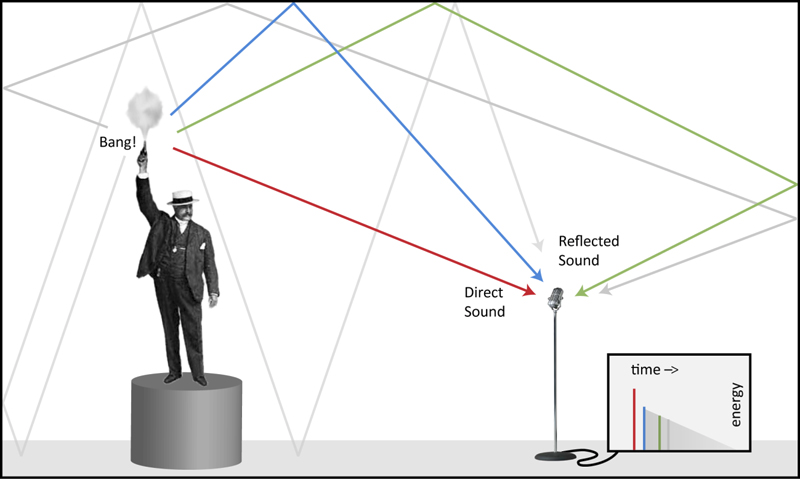
\includegraphics[width=.8\textwidth]{figures/rir_bang.png}

    \end{columns}

    \begin{center}
        % real RIR with part
        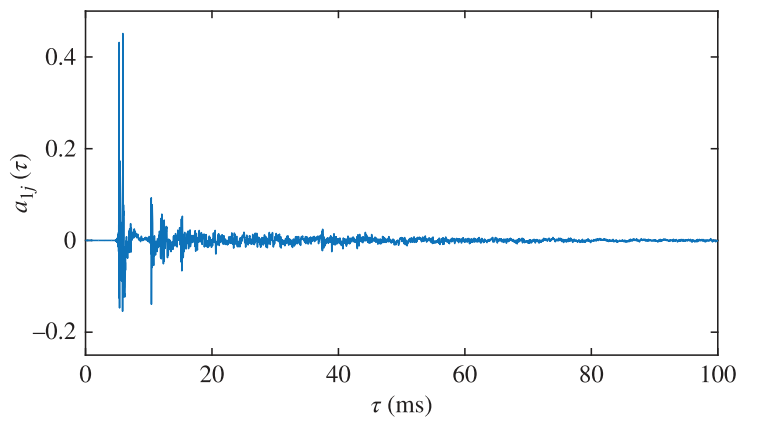
\includegraphics[width=0.8\textwidth]{figures/rir_measured.png}
    \end{center}

\end{frame}

\subsection{Current Challenges}

\begin{frame}{Problem Statement}
    Echoes can be modeled as sum of Dirac's delta function:

    \begin{equation*}
        \contRIR_i(t) =
            \textcolor{myred}{\contRIRidirect}(t) + \textcolor{myblue}{\contRIRiearly}(t) + \varepsilon_i(t)
            \approx \sum_{r=0}^{R} \ampir \delta\kparen{t - \textcolor{alert}{\tauir}} + \tikzmarknode{error}{\varepsilon}_i(t)
    \end{equation*}

    \begin{textblock*}{30mm}(100mm,35mm)
        \footnotesize
        \textcolor{gray}{\tikzmarknode{model}{models} later echoes, reverberation and other.}
    \end{textblock*}


    \begin{tikzpicture}[overlay,remember picture,
        nodes={inner sep=1pt, align=center, font=\footnotesize},
        gray!70,>=stealth] %
    \draw[->] (error.south) to[out=-90, in=180] (model.west);
    \end{tikzpicture}


    \begin{mydefblock}{Goals: Acoustic Echo Retrieval (AER)}
        Estimated $\set{\tauir, \textcolor{gray}{\ampir_i}}_{i,r}$
        from the microphone signals $\set{x_i}_i$
    \end{mydefblock}
    % \addendum{\scriptsize {Estimation of only $\tauir$ is known as TOAs estimation}}

    \begin{block}{Challenges:}
        \begin{itemize}
            \item RIRs depend on the scene geometry (room, source and mic position)
            \item Big under-modelling error (late reverberation and noise)
            \item In reality: $\ampir \to \ampir(t)$ due to
            \begin{itemize}
                \item due to air attenuation, wall absorption, ...
                \item due to sampling process
            \end{itemize}
        \end{itemize}
    \end{block}

    % \begin{center}
    %     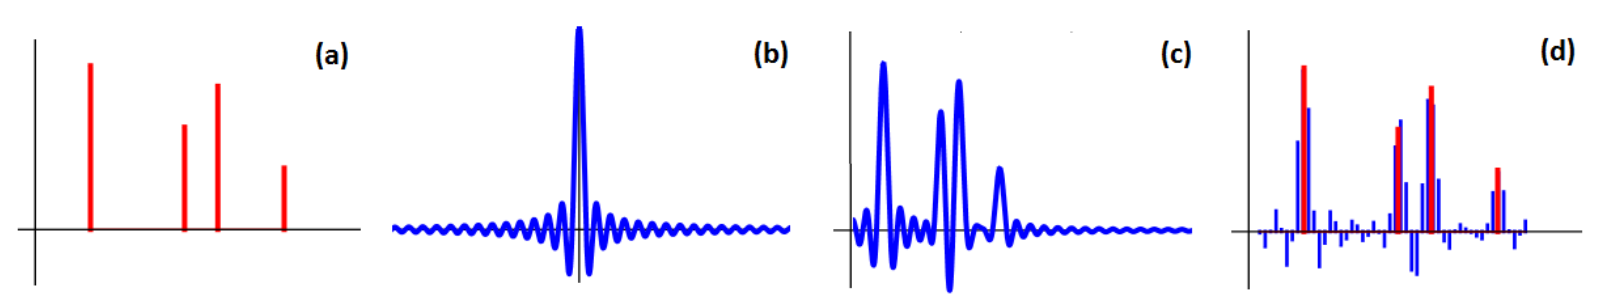
\includegraphics[width=0.8\textwidth]{figures/basismismatch.png}
    %     \\{\addendum{\scriptsize Courtesy of Helena Tukuljac~\cite{tukuljac2018mulan}}}
    %     \\{\small \textcolor{myred}{\iconAlert~sampling breaks sparsity and non-negativity}}
    % \end{center}

\end{frame}

    \section{Acoustic Echo Estimation}
    % \subsection*{State of The Art}

% \begin{frame}[t]{Acoustic Echo Retrieval \hfill\faBook}
%     \begin{columns}[T,onlytextwidth]
%         \column{0.55\textwidth}
%             Estimating early (strong) reflections for microphones recordings, i.e.,
%             \begin{equation*}
%                 \{\contMic_i\}_i \longrightarrow \{ \tauir, \textcolor{gray}{\ampir} \}_{i,r}
%             \end{equation*}
%         \column{0.4\textwidth}
%             \begin{figure}
%                 \centering
%                 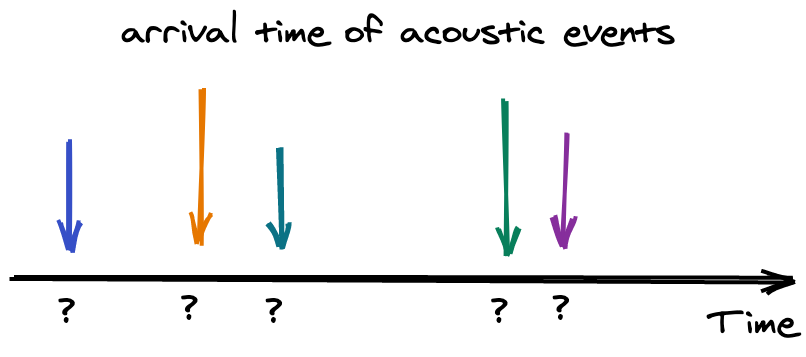
\includegraphics[width=\textwidth]{./figures/arrivals.png}
%             \end{figure}
%     \end{columns}

%     \vfill
%     \begin{columns}[T,onlytextwidth]
%         \column{0.48\textwidth}
%         \textbf{Scenarios:} the source signal is

%         \begin{center}
%             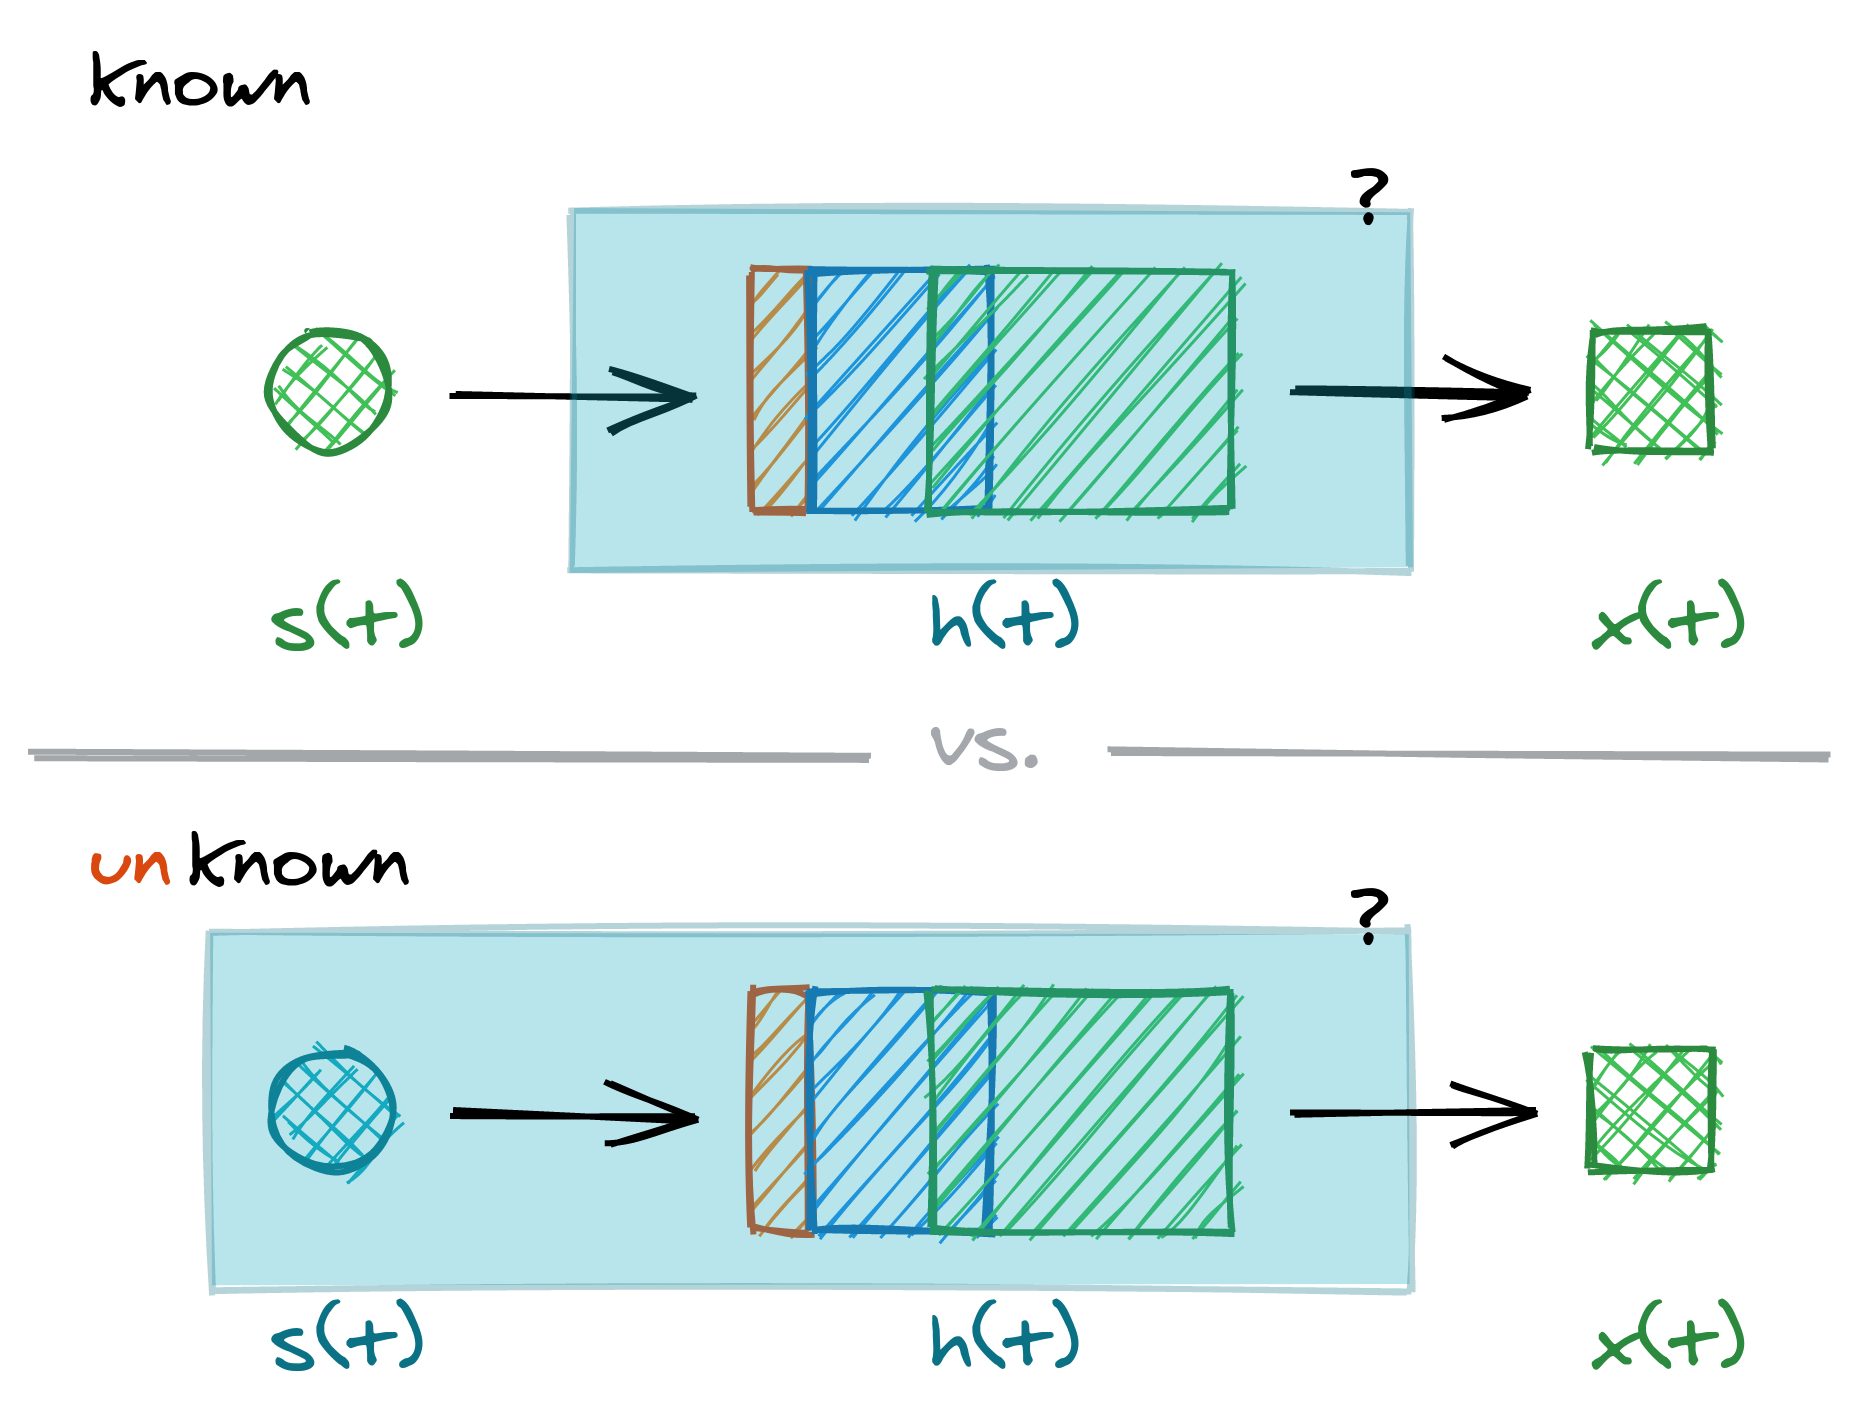
\includegraphics[width=.9\textwidth]{./figures/active-passive.png}
%         \end{center}

%         \only<4>{
%         \column{0.48\textwidth}
%         Active
%         \vspace{-2mm}
%         \begin{itemize}
%             \small
%             \item[\faEye] \textbf{non-blind} problem
%             \item[\faVolumeUp] \textbf{intrusive} or specific setups
%             % \item known emitted signal
%             % \item Time of Arrival (\textbf{TOA}s) accessible
%             % \\\hspace{.3em} $\implies$ \textbf{single} mic
%             \\\hspace{-1em}\addendum{\footnotesize \textbf{Application:} sonar, calibration, measurements, etc.}
%         \end{itemize}

%         \vspace{-5mm}
%         Passive
%         \vspace{-2mm}
%         \begin{itemize}
%             \small
%             \item[\faEyeSlash] \textbf{blind inverse} problem (harder)
%             \item[\faMicrophone] \textbf{passive} and more common setups
%             % \item \alert{un}knwon
%             % \item Time Difference of Arrivals (\textbf{TDOA}s) only
%             % \\\hspace{.3em} \textbf{multi-mic}
%             \\\hspace{-1em}\addendum{\footnotesize \textbf{Applications:} recording on smart speakers, laptop, etc.}
%         \end{itemize}
%         }

%         \only<5->{
%         \column{0.48\textwidth}
%         \centering
%         \textbf{Methods:} the estimation is
%         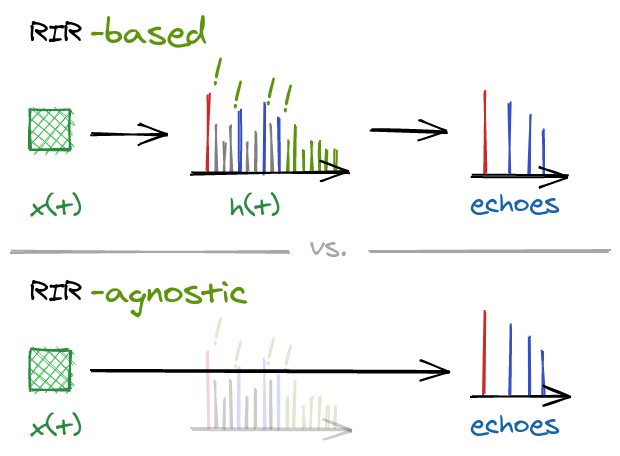
\includegraphics[width=.9\textwidth]{./figures/based-agnostic.png}
%         }
%     \end{columns}

%     \vfill
%     \textcolor{myred}{\textbf{Our case:} signal source and passive system of ($I$ microphones)}

% \end{frame}

% \begin{frame}[t]{\alert{Passive} Acoustic Echo Retrieval \hfill\faBook}

%         \vspace{.5em}
%         \begin{columns}[T,onlytextwidth] % align columns
%             \begin{column}{.48\textwidth}
%                 \textbf{RIR-\alert{based} approaches}
%             \end{column}
%             \begin{column}{.48\textwidth}
%                 \textbf{RIR-\alert{agnostic} approaches}
%             \end{column}%
%         \end{columns}

%         \vspace{.5em}
%         \begin{columns}[onlytextwidth] % align columns
%             \begin{column}{.48\textwidth}
%                 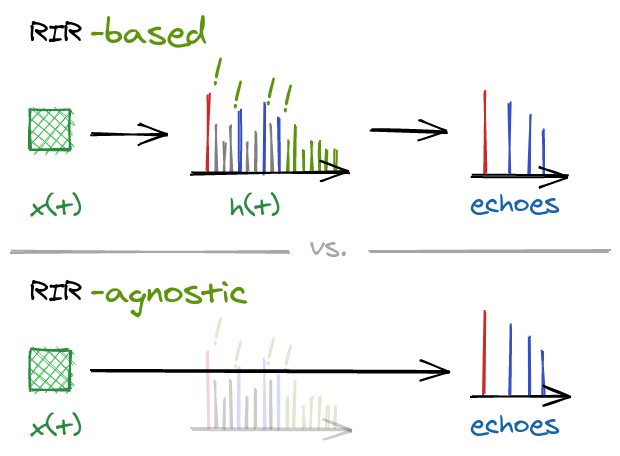
\includegraphics[trim={0 31em 0 7em},clip,width=.9\textwidth]{./figures/based-agnostic.png}
%             \end{column}
%             \begin{column}{.48\textwidth}
%                 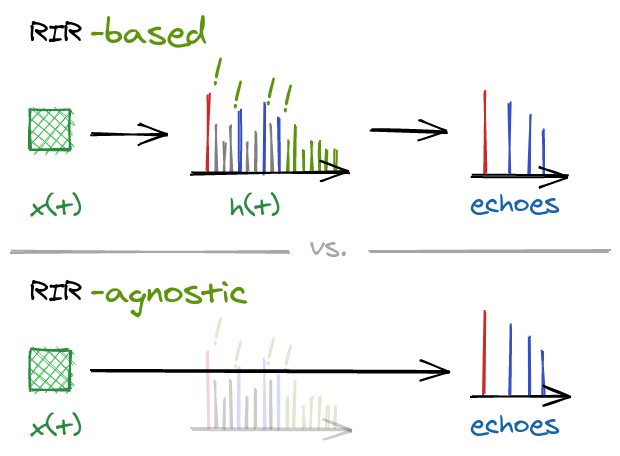
\includegraphics[trim={0 0 0 40em},clip,width=.9\textwidth]{./figures/based-agnostic.png}
%             \end{column}%
%         \end{columns}

%         \vspace{.5em}
%         \begin{columns}[T,onlytextwidth] % align columns
%             \begin{column}{.48\textwidth}
%                 \small
%                 \begin{enumerate}
%                     \item ``BCE''\footnotemark[1] problem $\implies$ RIRs
%                     \item Peak picking $\implies$ Echoes
%                 \end{enumerate}
%             \end{column}
%             \begin{column}{.48\textwidth}
%                 \small
%                 \begin{enumerate}
%                     \item Direct off-grid estimation of $\set{\tauir, \ampir}$
%                     e.g., with maximum-likelihood
%                     % \\\textcolor{gray}{(+ \small direction of arrivals can be used instead)}
%                 \end{enumerate}
%             \end{column}%
%         \end{columns}

%         \vspace{1em}
%         \begin{columns}[T,onlytextwidth] % align columns
%             \column{.48\textwidth}
%                 \small
%                 \begin{itemize}
%                     \item[\cmark] \pro{BCE is well and known studied}
%                     \item[\cmark] \pro{it is the state of the art}
%                     \\{\scriptsize~\cite{crocco2016estimation}}
%                     \item[\cmark] \pro{reasonably good for some application}
%                 \end{itemize}
%             \column{.48\textwidth}
%                 \small
%                 \begin{itemize}
%                     \item[\cmark] \pro{No full RIRs \& no peak picking}
%                     \begin{itemize}
%                         \item lower complexity
%                         \item less hyperparameters
%                     \end{itemize}
%                     \item[\cmark] \pro{Echo properties are respected}
%                     \\\addendum{\footnotesize e.g. Sparsity, Non-negativity}
%                     \end{itemize}
%         \end{columns}

%         \vspace{1em}
%         \begin{columns}[T,onlytextwidth] % align columns
%             \column{.48\textwidth}
%                 \small
%                 \begin{itemize}
%                     \item[\xmark] \con{Full RIRs need to be estimated}
%                     \item[\xmark] \con{Peak picking has hyperparameters}
%                     \item[\xmark] \con{Issues due to \textit{on-grid} estimation}
%                     \\[\footnotesize \faReply~next topic]
%                 \end{itemize}
%             \column{.48\textwidth}
%                 \small
%                 \begin{itemize}
%                     \item[\xmark] \con{exploratory \faWpexplorer}
%                     \\\addendum{no standard solver, few works on audio}
%                     % \item[\xmark] \con{no ``simple'' implementation}
%                     % \\\addendum{not standard math of BCE}
%                 \end{itemize}
%         \end{columns}

%     \footnotetext[1]{Blind Channel Estimation}

% \end{frame}

% \begin{frame}{Limitations \& bottleneck  \hfill\faBook}

%     \begin{block}{\faExclamationCircle~ Echoes are not necessarely ``on-grid''}

%         \vspace{-2mm}
%         \begin{itemize}
%             \item Sparsity and non-negativity not true ``on grid''
%             % We measure filters, not diracs

%             \item \emph{Body guard} effect \cite{duval2017sparse}
%             \begin{itemize}
%                 \item[$\rightarrow$] low recall $\implies$ low accuracy % (2 echoes instead of 1)
%                 \item[$\rightarrow$] slow convergence % bouncing between 2 echoes
%             \end{itemize}
%             \item Pick Picking
%             \begin{itemize}
%                 \item[$\rightarrow$] manually tuned / corrected
%             \end{itemize}
%         \end{itemize}
%     \end{block}

%     \begin{columns}[onlytextwidth]
%         \column{0.60\textwidth}

%         \begin{block}{How about higher sampling rate $F_s$?}

%             \vspace{-2mm}
%             \begin{itemize}
%                 \item[$\rightarrow$] Increase Precision
%             \end{itemize}
%         \end{block}

%         \begin{block}{But, computational bottleneck!}

%             \vspace{-2mm}
%             \begin{itemize}
%                 \item Bigger vectors and matrices
%                 \begin{itemize}
%                     \item[$\longrightarrow$] memory usage
%                 \end{itemize}
%                 \item the higher the sampling frequency
%                 \begin{itemize}
%                     \item[$\longrightarrow$] more ill-conditioned
%                 \end{itemize}
%             \end{itemize}
%         \end{block}

%         \column{0.38\textwidth}
%         \begin{center}
%             \textcolor{myred}{\textbf{How to address this?}}
%         \end{center}
%         \begin{mycontriblock}
%             RIR-agnostic + off-grid
%             \begin{enumerate}
%                 \item Deep Neural Network
%                 \item Continuous Dictionary
%             \end{enumerate}
%         \end{mycontriblock}

%     \end{columns}

%     \begin{textblock*}{40mm}(80mm,15mm)
%         \includegraphics<1->[width=\columnwidth]{figures/bodyguard.png}
%     \end{textblock*}

% \end{frame}

% \subsection{\lantern}

% \begin{frame}{Proposed approach: learning-based \& off-grid \hfill\faBrain}

%     % \textbf{Recall}: AER $\Leftrightarrow$ $\{\contMic_i\}_i \overset{?}{\longrightarrow} \{ \tauir, \textcolor{black!20}{\ampir} \}_{i,r}$
%     \begin{mydefblock}{Idea: (Deep) Learning-based AER}
%         \begin{enumerate}
%             \item Use \alert{virtually} supervised deep learning models
%             \item Estimate first echo (simple but important)
%             \item Only 2 microphones
%         \end{enumerate}
%     \end{mydefblock}

%     \vfill
%     \textbf{Motivations:}
%     \begin{itemize}
%         \item This \textit{direct} mapping is difficult, the \textit{inverse} ``is not''
%         \\$\rightarrow$ acoustic simulators:
%             $\text{mic/src/room geometry}
%             \; \longrightarrow \;
%             \set{\tauir,\ampir}, \; \contRIR_i, \quad \contMic_i$
%         \item Acoustic simulator are ``simple'', versatile and fast
%         \\$\to$ many data
%         \item This approach is successful in \textit{Sound Source Localization}
%         \\$\to$ position is related to echoes
%         \\{\small\cite{kataria2017hearing,nguyen2018autonomous,perotin2019regression} \textcolor{myred}{\faExclamationTriangle~Not only DNN}}
%     \end{itemize}

% \end{frame}

% \begin{frame}{Proposed approache: models \hfill\faBrain}

%     \begin{columns}[T,onlytextwidth]
%         \column{0.48\textwidth}
%         \textbf{Inputs:}
%         {\small Interchannel level and phase difference features\footnotemark[1] from
%             \[ \footnotesize
%             R[f] = \timeavg \frac{X_2[f,t]}{X_1[f,t]}
%             \approx \timeavg \frac{H_2[f]\alert{S[f,t]}}{H_1[f]\alert{S[f,t]}}
%             \]
%             \\$\approx$ the relative transfer function
%             \\$\to$ remove source dependency
%         }

%         \column{0.48\textwidth}
%         \textbf{Output:} {\small Inter and intra arrival delays}
%         \begin{columns}
%             \column{0.60\textwidth}
%             \includegraphics<1>[width=\textwidth]{figures/lantern_rir_tdoa1(1).png}%
%             \includegraphics<2>[width=\textwidth]{figures/lantern_rir_tdoa1(2).png}%
%             \includegraphics<3->[width=\textwidth]{figures/lantern_rir_tdoa1(3).png}%
%             \column{0.45\textwidth}
%             \footnotesize
%             \centering
%             4 TOA
%             \\$\downarrow$
%             \\3 Time \alert{Difference} of Arrivals (\alert{\textbf{TDOAs}})\footnotemark[1]
%         \end{columns}
%         \begin{center}
%             \small
%             \textbf{HP:} first $\Leftrightarrow$ strongest echo
%         \end{center}
%     \end{columns}

%     \pause[4]
%     \vfill
%     \begin{itemize}
%         \item Architecture: $\MLP$, $\CNN$~{\footnotesize\cite{chakrabarty2017broadband,nguyen2018autonomous}}
%         \item Loss Function:
%         \begin{enumerate}
%             \item RMSE (Multi-label regression) $\to$ TDOAs
%             \item Gaussian log-likelihood $\to \kbrace{\mu_\tau, \sigma^2_\tau} \;\forall \tau \in$ TDOAs \hspace{1em}\tikzmark{CNN}\tikzmark{CNNtop}
%             \item Student log-likelihood $\to \kbrace{\mu_\tau, \lambda_\tau, \nu_\tau} \;\forall \tau \in$ TDOAs \tikzmark{CNNbot}
%         \end{enumerate}

%         \pause[6]
%         \item Data:
%         \begin{itemize}
%             \item Virtually-supervised learning (= data from acoustic simulator)
%             \item white-noise as source signal + noise
%             \item 2 microphone in close-surface scenario
%         \end{itemize}
%     \end{itemize}

%     \visible<5->{
%     \begin{tikzpicture}[overlay, remember picture]
%         \node[anchor=base] (a) at (pic cs:CNNtop) {\vphantom{h}}; % push the mark to the top of the line (ie including ascenders)
%         \node[anchor=base] (b) at (pic cs:CNNbot) {\vphantom{g}}; % push the mark to the bottom of the line (ie including descenders)
%         \draw [decoration={brace,amplitude=0.35em},decorate,thick,gray]
%             (a.north -| {pic cs:CNN}) -- node[right,inner sep=1em] {
%                 \small \parbox{12em}{Good for data fusion\\Similar to \textbf{MDN}\\~{\footnotesize\cite{bishop1994mixture}}}
%                 } (b.south -| {pic cs:CNN});
%     \end{tikzpicture}
%     }

%     \visible<1->{
%         \footnotetext[1]{\tiny $\mathtt{ILD} = \log\kvbar{R}$, $\mathtt{IPD} = \arg{R/\kvbar{R}}$}
%     }

% \end{frame}

% \begin{frame}{\faFlask~Experimental results \hfill\faBrain}

%     \vspace{2mm}
%     \begin{mycontriblock}
%         \textbf{Proposed Method:} $\MLP$, $\CNN$, $\CNNn$, $\CNNt$
%     \end{mycontriblock}
%     \begin{mysotablock}
%         \textbf{Baseline:} $\GCCPHAT${\tiny~\cite{knapp1976generalized}}
%     \end{mysotablock}

%     \textbf{Metrics:} normalized RMSE (0 = best fit, 1 = random fit)

%     % \vspace{2mm}
%     % \begin{columns}[T,onlytextwidth]

%     %     \column{0.32\textwidth}
%     %     Are better than baseline?
%     %     \\\addendum{\footnotesize only TDOA on direct path}
%     %     \\\hspace{.3em}$\to$ yes \cmark

%     %     \column{0.32\textwidth}
%     %     Echoes' \alert{TDOAs}?
%     %     \\\hspace{.3em}$\to$ yes \cmark
%     %     \\\hspace{.3em}$\to$ CNN better than MLP

%     %     \column{0.32\textwidth}
%     %     Are robust to noise?
%     %     \\\hspace{.3em}$\to$ yes \cmark
%     %     \\\hspace{.3em}$\to$ \CNNn/\CNNt better than \CNN

%     % \end{columns}

%     \begin{center}
%         \includegraphics<1>[trim={0 30 0 0},clip,height=0.33\textwidth]{figures/lantern_snr1.pdf}%
%         \includegraphics<2>[trim={0 30 0 0},clip,height=0.33\textwidth]{figures/lantern_snr2.pdf}%
%         \includegraphics<3>[trim={0 30 0 0},clip,height=0.33\textwidth]{figures/lantern_snr3.pdf}%
%         \includegraphics<4->[trim={0 30 0 0},clip,height=0.33\textwidth]{figures/lantern_snr4.pdf}%
%     \end{center}

%     \vspace{-3mm}
%     \visible<2->{\textbf{Observation:}}

%     \vspace{-2mm}
%     \begin{itemize}\small
%         \item<2->[\cmark] $\MLP$ outperforms $\GCCPHAT$ on TDOA estimation
%         \item<3->[\cmark] $\CNN$ outperforms $\MLP$ (lower error and smaller variance)
%         \item<4->[\cmark] $\CNNn$ and $\CNNt$ outperform $\CNN$ (lower error and smaller variance)
%         \item<4->[\xmark] TDOA between DP and 1$^\text{st}$ echo more difficult
%         \item<5->[\xmark] In general, only the first echo on white noise
%     \end{itemize}

% \end{frame}


\subsection{\blaster}

\begin{frame}{State of the Art \hfill\faBook}

    \begin{block}{Key ingredient -- \textit{Cross relation identity}}

        \vspace{-3mm}
        \begin{columns}[onlytextwidth]
        \column{0.6\textwidth}
            \begin{align*}
                \contMic_1 &= \contRIR_1 \contConv \contSrc
                \\\contRIR_2 \contConv \contMic_1 = \textcolor{gray}{\contRIR_2 \contConv \contRIR_1 \contConv \contSrc}
                    &\textcolor{gray}{= \contRIR_1 \contConv \contRIR_2 \contConv \contSrc} = \contRIR_1 \contConv \contMic_2
            \end{align*}

            \column{0.3\textwidth}
            \centering
            \only<1>{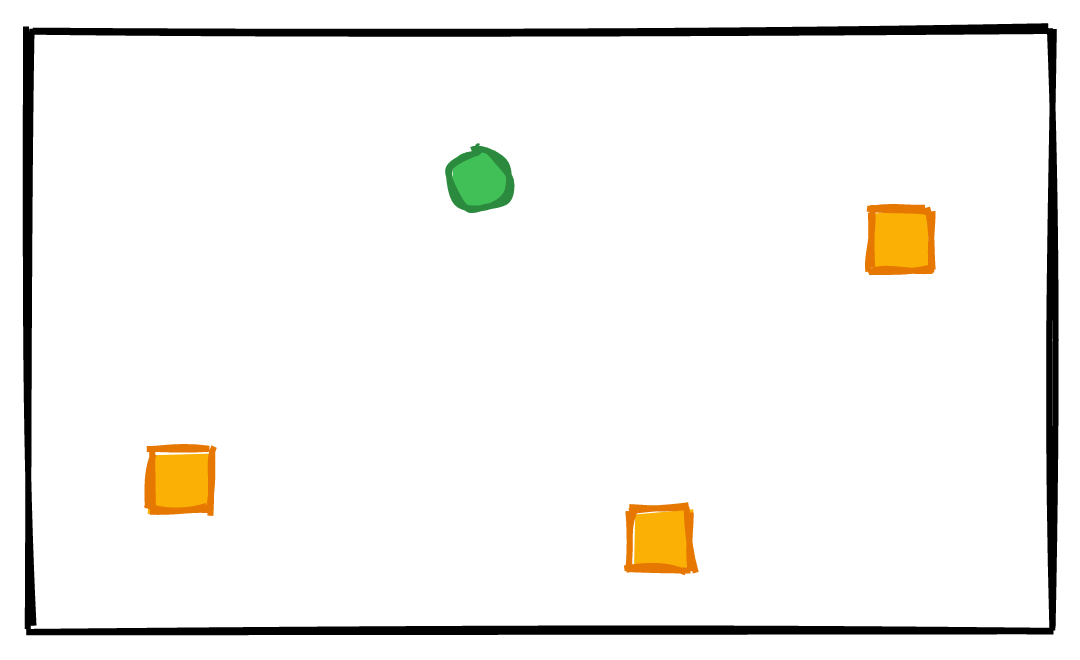
\includegraphics[width=0.9\textwidth]{figures/xrelation1.png}}%
            \only<2->{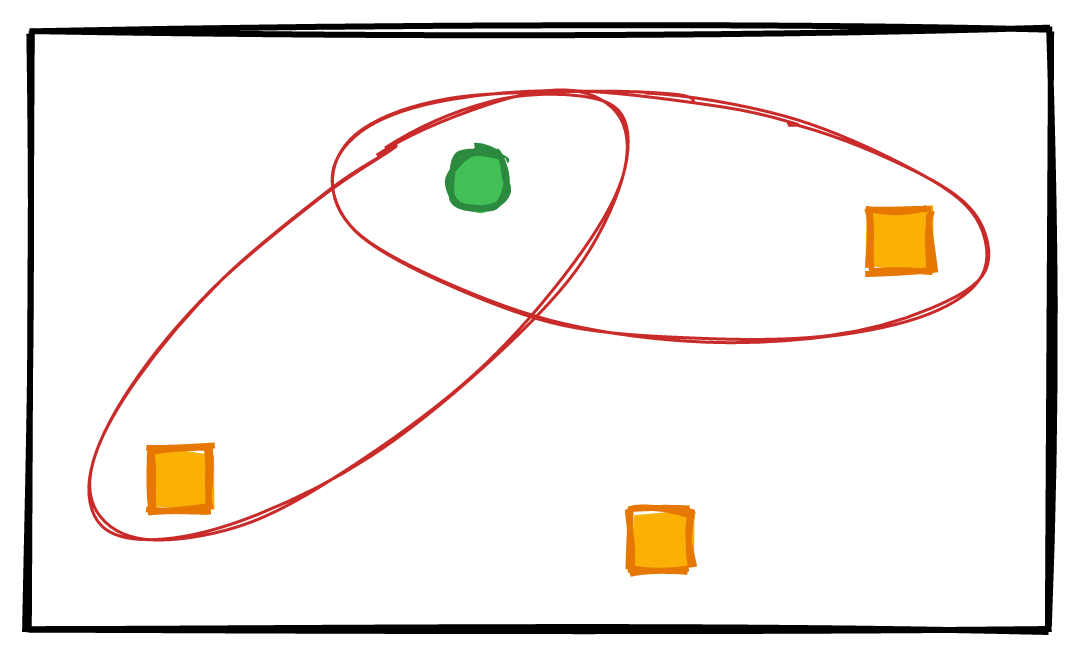
\includegraphics[width=0.9\textwidth]{figures/xrelation2.png}}
        \end{columns}
    \end{block}

    \begin{block}{Ideas:}
    \begin{enumerate}
        \small
        \item Sampled version of $\contMic_1,\contMic_2$ are available: $\discMic_1, \discMic_2$
        \item Echo TOAs $\propto$ sampling frequency
        \item Find echoes $\rightarrow$ \textbf{find sparse vectors} $\discRIR_1, \discRIR_2$ of length $L$
        \item Modeled as \textbf{Lasso}-like problem

        \vspace*{2mm}
        \begin{mysotablock}
            \begin{equation*}
                \widehat{\discRIR}_1, \widehat{\discRIR}_2 \in
                \underset{\discRIR_1, \discRIR_2\in\kR^n}{\arg\min}\;
                \Vert \discMic_1 \contConv \discRIR_2 - \discMic_2 \tikzmarknode{conv}{\contConv} \discRIR_1 \Vert_2^2
                + \lambda \mathcal{P}(\discRIR_1, \discRIR_2)
                \quad\text{s.t.}\quad\mathcal{C}(\discRIR_1, \discRIR_2)
            \end{equation*}

            \vspace*{-2mm}
            \begin{center}
                \footnotesize
                $\mathcal{P}(\discRIR_1, \discRIR_2)$ $\longrightarrow$ sparse promoting regularizer
                \hspace{5mm} \footnotesize $\mathcal{C}(\discRIR_1, \discRIR_2)$ $\longrightarrow$ constraints e.g. \parbox{6em}{nonnegativity\\anchor}
            \end{center}
        \end{mysotablock}
        \begin{tikzpicture}[overlay,remember picture, %
            nodes={inner sep=1pt, align=center, color=gray, font=\footnotesize}, %
            gray,>=stealth] %
            \draw[->] (conv.north) to[out=90, in=180] ++ (+10mm,+4mm) node[right] %
            {{= $\mathtt{Toeplitz}(\discMic_i) \discRIR_j \in \mathcal{O}(L^2)$}};
        \end{tikzpicture}
    \end{enumerate}
    \end{block}

    \vspace{-12mm}
    \begin{block}{}
        \begin{center}
            \footnotesize
            \textcolor{mygreen}{\cmark}  \cite{tong1994blind} \qquad \textcolor{mygreen}{\cmark}  \cite{lin2008blind} \qquad \textcolor{mygreen}{\cmark} \cite{aissa2008blind} \\
            \textcolor{mygreen}{\cmark} \cite{kowalczyk2013blind} \qquad \textcolor{mygreen}{\cmark} \cite{crocco2016estimation}
        \end{center}
    \end{block}

 \end{frame}


\begin{frame}{Proposed approach: analytical \& off-grid \hfill\faJediOrder}

    \begin{block}{\textbf{Observation 1:} the cross relation remains true in the frequency domain}
        \begin{equation*}
            \mathcal{F}x_1 \cdot \mathcal{F}h_2 (\sfrac{n}{F_s}) = \mathcal{F}x_2 \cdot \mathcal{F}h_1(\sfrac{n}{F_s}) \qquad n=0\dots N-1
        \end{equation*}
        \end{block}

        \vspace{.5em}

        \pause
        \begin{block}{\textbf{Observation 2:} $\mathcal{F}\delta_{\mathrm{echo}}$ is known in closed-form}
        \end{block}

        \pause
        \vspace{1.em}
        \begin{block}{\textbf{Observation 3:} $\mathcal{F}{\mathrm{x_i}}$ can be (well) approximated by DFT}
        \begin{equation*}
            \mathbf{X}_i = \texttt{DFT}(\discMic_i) \simeq  \mathcal{F}{\discMic_i}(nF_s) \qquad n=0\dots N-1
        \end{equation*}
        \end{block}


        \pause
        \vfill
        \setbeamercolor{block title}{fg=white,bg=darkblue}
        \setbeamercolor{block body}{fg=black,bg=bluegreen!10}
        \begin{block}{\textbf{Idea:} Recover echoes by matching a finite number of frequencies}
        \begin{equation*}
            \underset{h_1,h_2 \in \substack{\text{measure} \\ \text{space}}}{\arg\min} \;
            \tfrac{1}{2} \kvvbar{
                \mathbf{X}_1 \cdot \mathcal{F}h_2 (f) - \mathbf{X}_2 \cdot \mathcal{F}h_1(f)
            }_2^2
            + \lambda \kvvbar{h_1 + h_2}_{\mathrm{TV}}
            \quad
            \text{s.t.}\;
            \begin{cases}
                h_1(\{0\})=1 \\
                h_l \geq 0
                \end{cases}
        \end{equation*}
        \end{block}

        \pause
        \begin{center}
            $\sim$ \textbf{Lasso} problem, but $\mathcal{F}h_2 (f)$ is a continuous function.
            \\Instance of a \textbf{BLasso} problem~\cite{bredies2020sparsity}
            \\Solved with Sliding Frank-Wolfe algorithm \cite{denoyelle2019sliding}
        \end{center}

        \begin{center}
            \textcolor{mygreen}{\cmark{no Toeplitz matrix} \qquad
            \cmark \, \parbox{8.5em}{Solutions is \\ a train of Dirac} \qquad
            \cmark \, \parbox{8em}{anchor prevents \\ trivial solution}}
        \end{center}

        % In the manuscript:
        % \begin{itemize}
        %     \item From Lasso to BLasso
        %     \item Pseudocode of the Algorithm
        %     \item How to manually tuned lambda
        % \end{itemize}
\end{frame}

\begin{frame}[t]{\faFlask~Experimental results \hfill\faJediOrder}
    % \begin{block}{Scenario}
    %     \begin{itemize}
    %         \item simulation data with ISM with Pyroomacoustics
    %         \item 1 source, 2 microphones, random room geometry
    %         \item Full RIRs
    %         \item 2 sources: broadband and speech
    %         \item 2 datasets: different SNR, different RT60
    %     \end{itemize}
    % \end{block}
    \begin{columns}[onlytextwidth]
        \begin{column}{0.45\textwidth}
            \begin{block}{Methods}
                \begin{itemize}
                    \item BSN --- SIMO BCE\cite{lin2007blind}
                    \item IL1C: iteratively-weighted $\ell_1$ constraint SIMO BCE
                    \\\cite{crocco2015room}
                    \item \blaster: Proposed off-grid approach
                \end{itemize}
            Baseline method are xvalidated on other dataset
            \end{block}
        \end{column}

        \begin{column}{0.45\textwidth}
            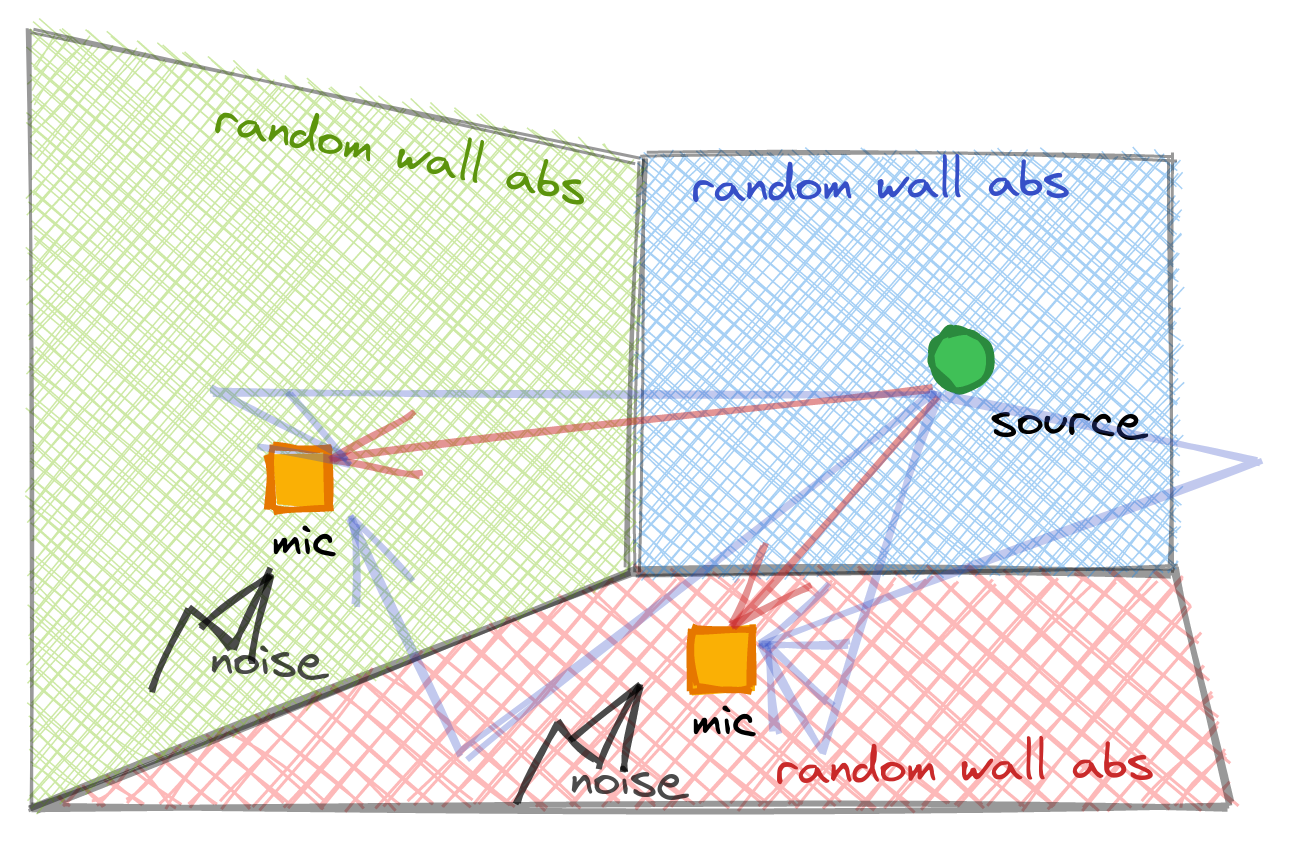
\includegraphics[width=0.9\textwidth]{figures/aer_scenario4.png}
        \end{column}
    \end{columns}

    \pause
    \begin{block}{Dataset}
        \begin{itemize}
            \footnotesize
            \item $\mathcal{D^{\text{SNR}}}$: $SNR \in [0, 20]$ dB, $\text{RT}_{60} = 400$ ms
            \item $\mathcal{D^{\text{RT60}}}$: $\text{RT}_{60} = [100, 1000]$ ms, $SNR = 20$ dB
        \end{itemize}
    \end{block}

    \pause
    \begin{block}{Metrics}
        \begin{itemize}
            \item Precision (how many estimated echoes are correct)
            \item RMSE (error on the correct guess)
        \end{itemize}
    \end{block}

\end{frame}


\begin{frame}<1>[label=echoes]{Performance per \# of echoes \hfill\faJediOrder}
    \begin{figure}[t!]
    \centering
        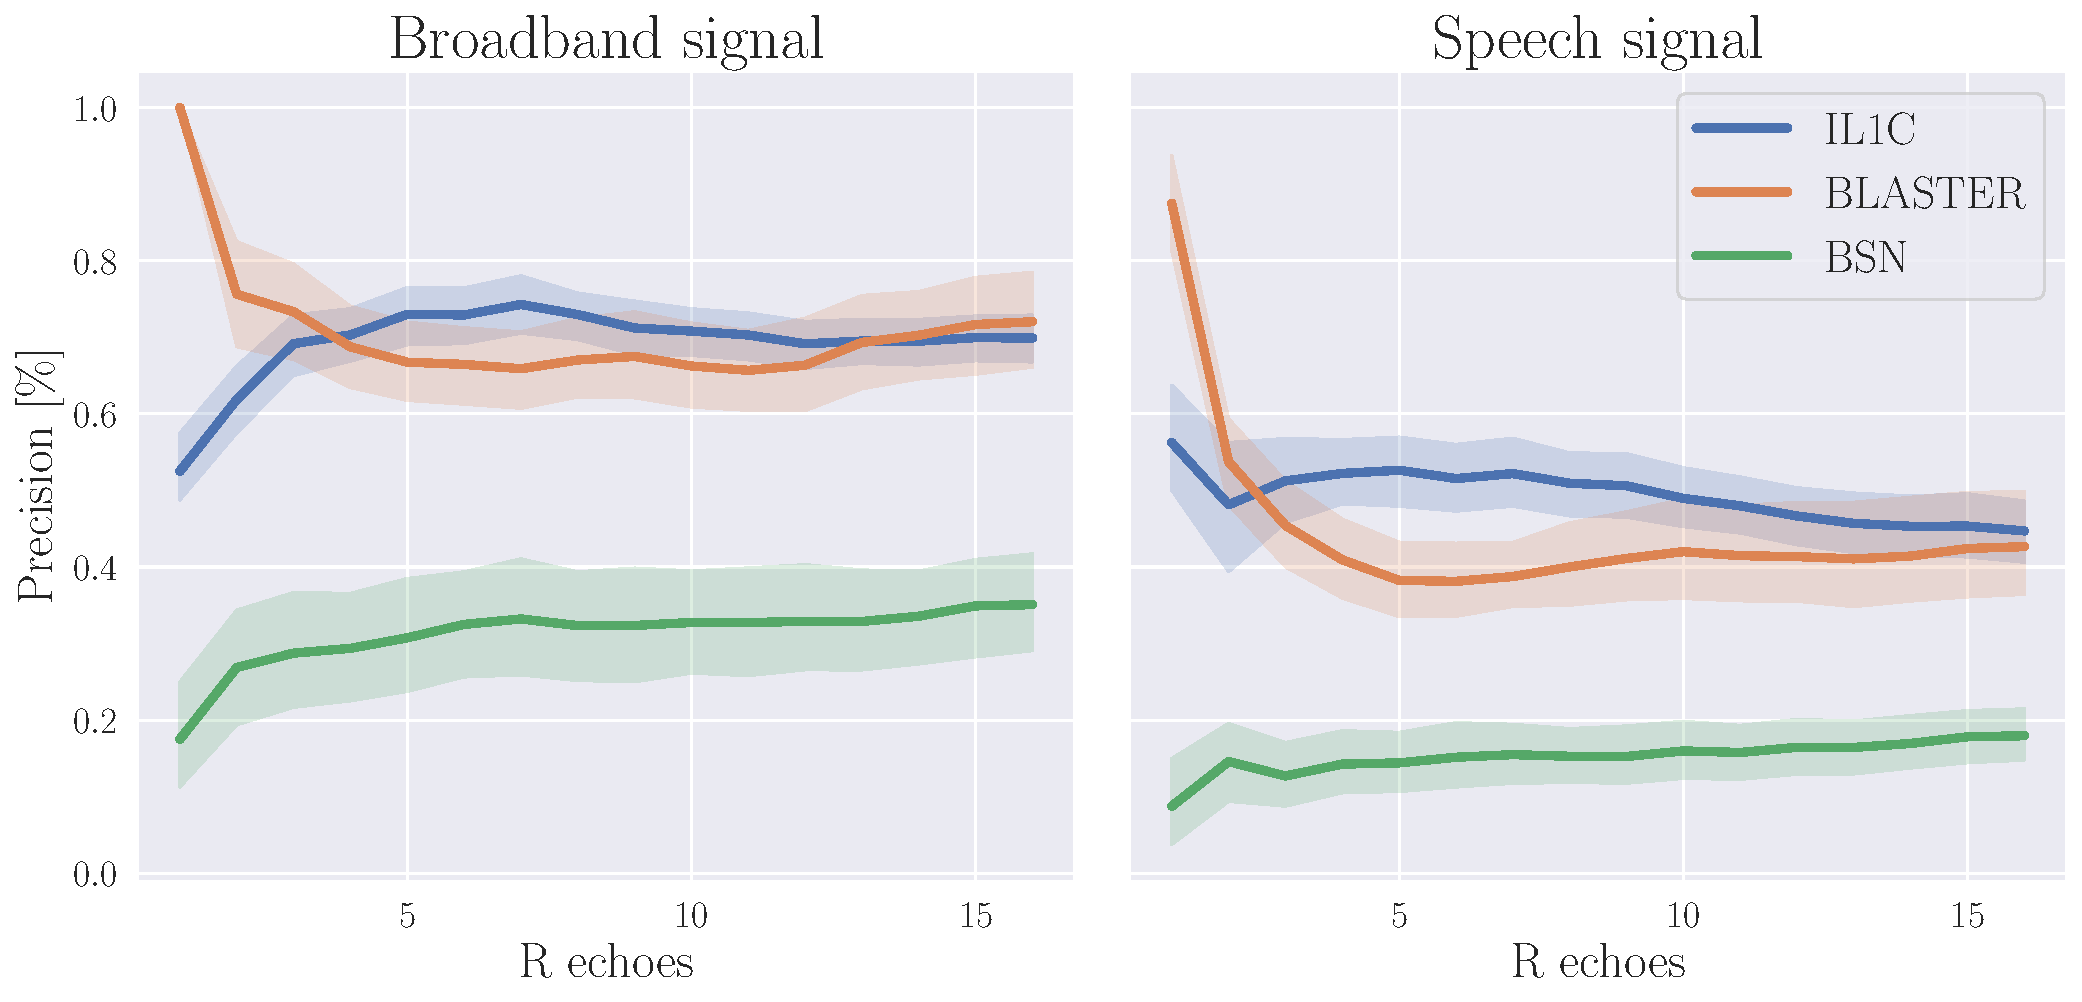
\includegraphics[width=\linewidth]{figures/p_k-7_thr-2_bns_crocco_blaster-peak_withRechoes.pdf}
        \caption{$\text{RT}_{60} = 400$ ms and SNR = 20 dB.}
    \end{figure}

    \begin{center}
        \textcolor{myred}{\xmark \: \parbox{8em}{Sensitive\\to \# echoes}}
        \textcolor{myred}{\xmark \: \parbox{8em}{Sensitive\\source signal}}
        \only<1>{
        \textcolor{mygreen}{\cmark \: \parbox{8em}{Good\\for 2 echoes}}
        }
        \only<2>{
        \textcolor{mygreen}{
        \cmark \: \parbox{8em}{Good\\for 2 echoes
                                    \\\cite{scheibler2018separake,di2019mirage}}}
        }
    \end{center}

\end{frame}

\againframe<2>{echoes}

\begin{frame}{Error per Dataset/Signal while recovering 7 echoes \hfill\faJediOrder}

    \begin{center}
        \begin{overpic}[width=0.8\textwidth]{figures/e_k-7_thr-2_bns_crocco_blaster.pdf}
            \put (102, 48){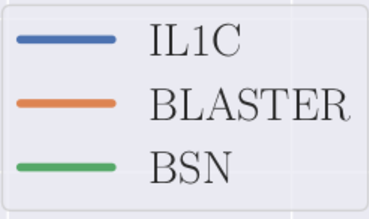
\includegraphics[width=5em]{figures/legend.pdf}}
        \end{overpic}
    \end{center}

    \begin{center}
        \textcolor{mygreen}{\cmark{Lower RMSE}} \qquad
        \textcolor{mygreen}{\cmark \, \parbox{8.5em}{Robustness\\
        to SNR and $\text{RT}_{60}$}} \qquad
        \textcolor{myred}{\xmark \, \parbox{8em}{Source signal\\dependent}}
    \end{center}

\end{frame}


% % \subsection{Interim conclusion (2/4)}

% % \begin{frame}{Interim conclusion (2/4)}
% %     \begin{block}{on Acoustic Echo Retrieval:}
% %         \begin{itemize}
% %             \item Most of the literature is on Passive and RIR-based, with on-grid approaches
% %             \item On-grid approaches suffers by the off-grid nature of the echoes (complexity, sampling)
% %         \end{itemize}
% %     \end{block}

% %     \begin{block}{on \blaster:}
% %         \begin{itemize}
% %             \item[\cmark] off-grid parameter-free which exploit dirac closed-form model (non negativity and sparsity)
% %             \item[\cmark] smaller RMSE due to super-resolution, better for small \# of echoes
% %             \item[\xmark] source dependent and on number of echoes
% %             \item[\xmark] validate only on synthetic data
% %             \item[$\rightarrow$] Multichannel and RTF-based extention
% %         \end{itemize}
% %     \end{block}

% %     \begin{block}{on \lantern:}
% %         \begin{itemize}
% %             \item[\cmark] promising results for first echo estimation
% %             \item[\cmark] direct application for table top application
% %             \item[\xmark] difficult extention
% %             \item[\xmark] need for real data validation
% %             \item[$\rightarrow$] physically-constrained neural network
% %             \item[$\rightarrow$] missing frequencies in the input
% %         \end{itemize}
% %     \end{block}
% % \end{frame}

    \section{Echo-aware Application}
    \subsection{introduction}

\begin{frame}{Audio signal processing and sound propagation}
    \begin{block}{Sound propagation is}

        \begin{columns}[onlytextwidth]

            \begin{column}{.48\textwidth}
                \begin{itemize}
                \item completely ignored
                \item assumed free-field case (\textit{anechoic})
                \item model it full (\textit{reverberant})
                \item \textit{learned} it full (\textit{reverberant})
                \item model few early echoes (\textit{multipath})
            \end{itemize}
            \end{column}

            \begin{column}{.48\textwidth}
                \centering
                \only<1>{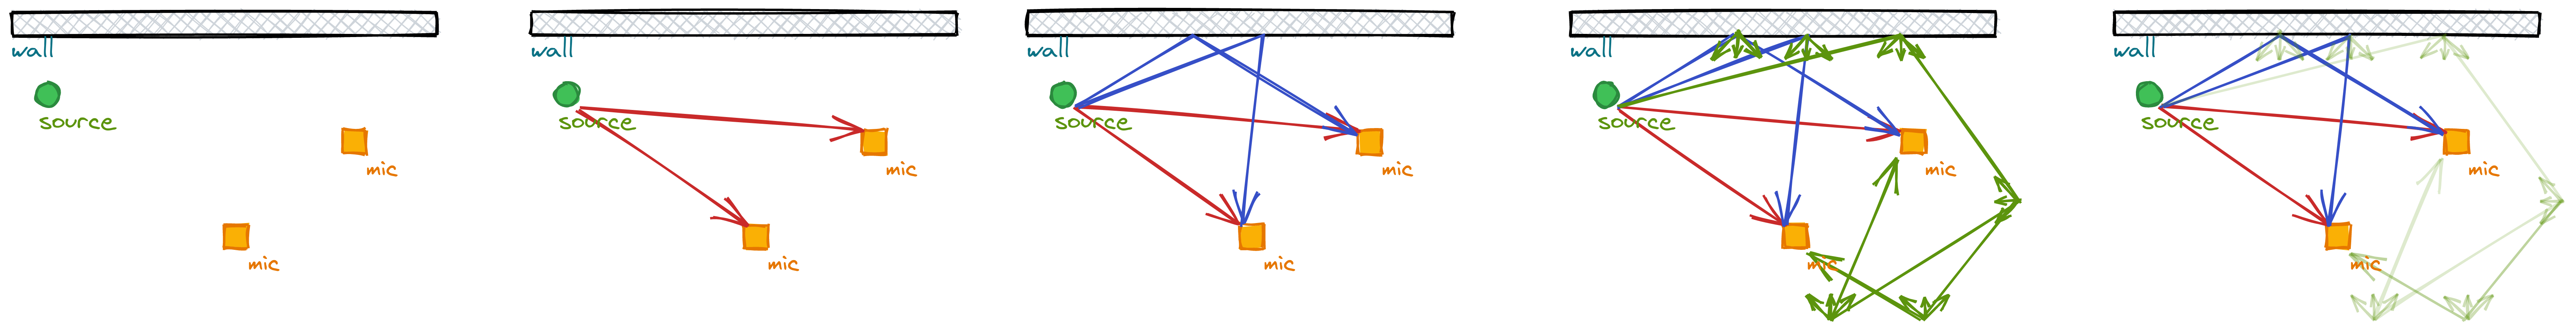
\includegraphics[trim={0 0 680em 0},clip,width=.8\textwidth]{figures/prop_it.png}}
                \only<2>{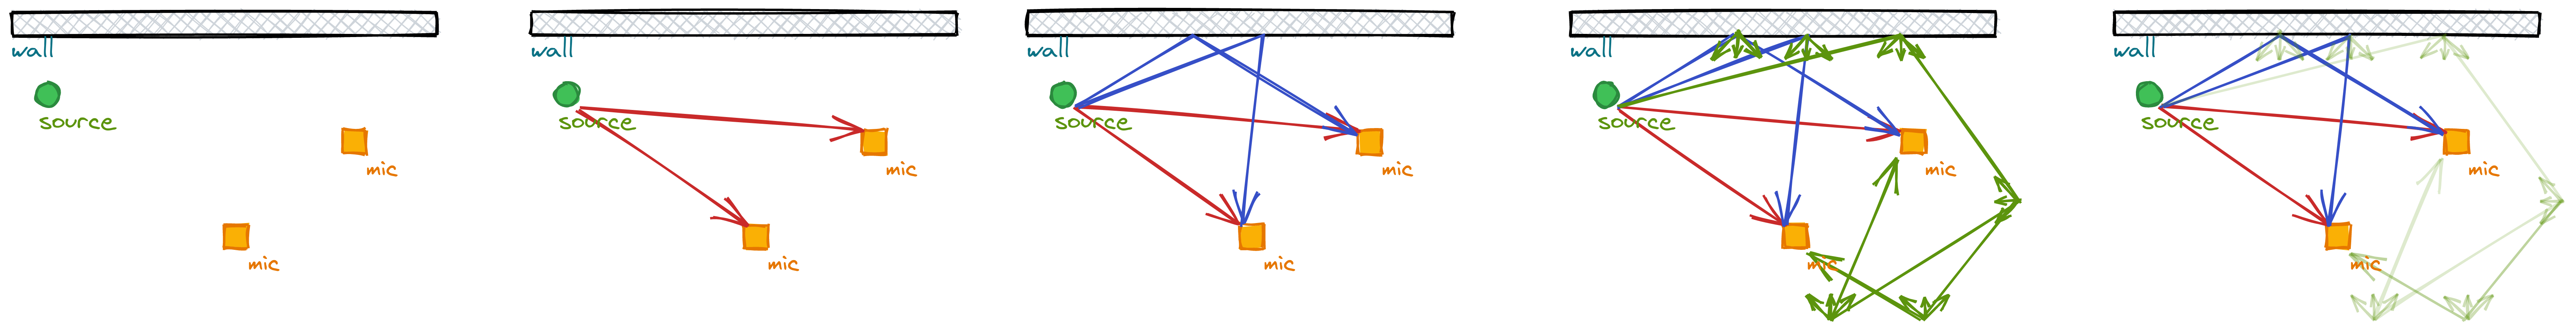
\includegraphics[trim={670em 0 5em 0},clip,width=.8\textwidth]{figures/prop_it.png}}

                \vspace{-2.3em}
                \begin{equation*}
                    \begin{aligned}
                        x_i(t) &= (h_i \ast s)(t)\\
                        h_i( t) &= \textcolor{myred}{h_i^d(t)} + \textcolor{myblue}{h_i^e(t)} + \textcolor{mygreen}{h_i^r(t)}
                    \end{aligned}
                \end{equation*}
            \end{column}

        \end{columns}
    \end{block}

    % \begin{alertblock}{$\Leftarrow$ \textbf{strong early reflection} and \textbf{strong reverberation} level}
    %     \begin{itemize}
    %         \item detrimentally affect typical Audio Scene Analysis algorithm
    %         \item undesired interfering source
    %         \item undesired position of the true sources (TDOA disambiguation)
    %     \end{itemize}

    % \end{alertblock}
    \begin{block}{Recall}
        \begin{itemize}
            \item anechoic case: easy mapping, but incoherence or wrong processing
            \item reverberant case: difficult mapping and estimation, but coherent processing
        \end{itemize}
        \hfill \textcolor{myred}{\textbf{What can we do with echoes?}}
    \end{block}
\end{frame}

\begin{frame}{Echo-aware Application}

    \begin{block}{Echoes = same content, different time/direction}
        \centering
        \adjincludegraphics[Clip={0\width} {0\height} {.66\width} {0\height},width=0.6\textwidth]{figures/echo_aware.png}
    \end{block}


    Echoes helps indoor processing:
    \begin{columns}[T,onlytextwidth]
        \column{.32\textwidth}
        \begin{block}{\textbf{What?}}
            \small
            Echoes = repetitions
            \begin{itemize}
                \item
                \only<1>{Sound Source Separation}
                \only<2>{\alert{Sound Source Separation}}
                \item Speech Enhancement
                \\\textcolor{gray}{\small(Dereverberation, Denoising, Room Equalization)}
            \end{itemize}
        \end{block}

        \column{.32\textwidth}
        \begin{block}{\textbf{Where?}}
            \small
            Echoes $\in$ indoor propagation
            \begin{itemize}
                \item Sound Source Localization
                \item Microphone Calibration
                \item Room Geometry Reconstruction
            \end{itemize}
        \end{block}

        \column{.32\textwidth}
        \begin{block}{\textbf{How?}}
            \small
            Echoes $\in$ sound propagation
            \begin{itemize}
                \item Blind Channel Estimation
                \item Acoustic Measurements
            \end{itemize}
        \end{block}
    \end{columns}
\end{frame}

\subsection{mirage}

\begin{frame}{\mirage - Sound Source Locatization with Echoes}

    \vspace*{5mm}
    \begin{columns}

        \begin{column}{0.5\textwidth}
            \begin{block}{The \alert{Picnic} Scenario:}
                \begin{itemize}
                    \small
                    \item One source
                    \item Two microphones
                    \begin{itemize}
                        \item[$\rightarrow$] passive scenario
                        \item[$\rightarrow$] generalizable later
                    \end{itemize}
                    \item Close to a very reflective surface
                    \begin{itemize}
                        \item[$\rightarrow$] First echo = Strongest echo
                        \item[$\rightarrow$] $\alpha_\text{picnic}$ const. $\forall f$
                        \item[$\rightarrow$] table-top device
                    \end{itemize}
                \end{itemize}
            \end{block}
        \end{column}

        \begin{column}{0.5\textwidth}
            \centering
            \only<1>{\adjincludegraphics[Clip={0\width} {0\height} {.5\width} {0\height},width=0.9\textwidth]{figures/mirage.png}}
            \only<2>{\adjincludegraphics[Clip={0.5\width} {0\height} {0\width} {0\height},width=0.9\textwidth]{figures/mirage.png}}
        \end{column}
    \end{columns}

    \vfill

    \begin{columns}

        \begin{column}{0.5\textwidth}
            \begin{block}{How to access the \textit{image} microphones?}
                \\$\implies$ each pair is augmented with echoes
            \end{block}
            \begin{center}
                \textcolor{myred}{\textbf{Mirage Array}}
            \end{center}

            idea: use SSL algorithm on this augmented array
            \\recall: echoes are known
        \end{column}

        \begin{column}{0.5\textwidth}
            \centering
            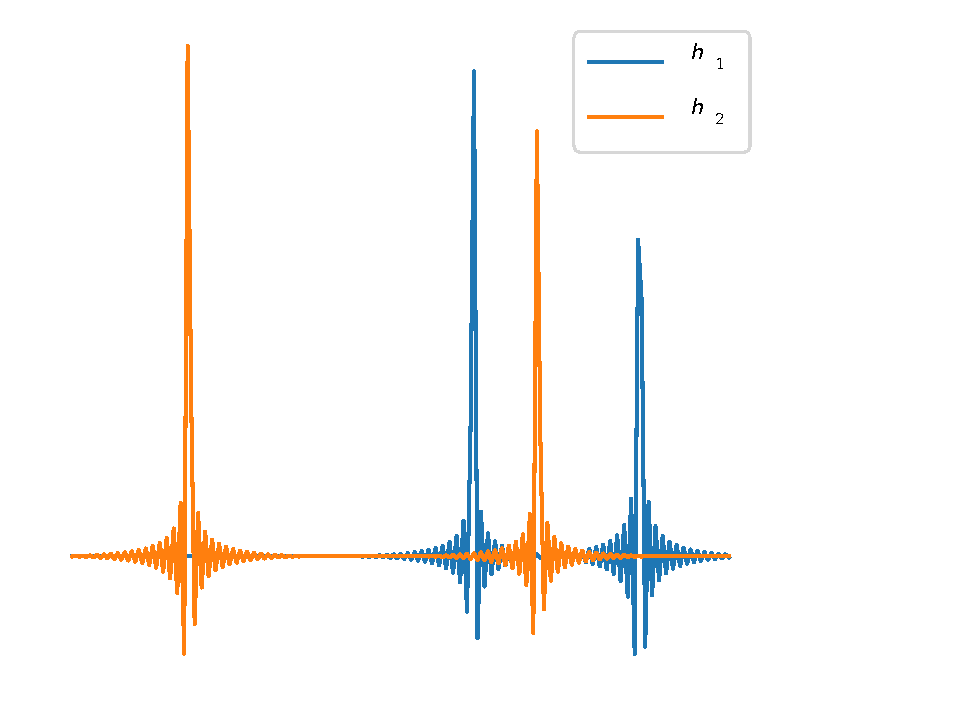
\includegraphics[width=\textwidth]{figures/rirs1.pdf}
        \end{column}
    \end{columns}


\end{frame}

\begin{frame}{\mirage - Sound Source Locatization with Echoes}

    \begin{columns}
        \column{0.6\textwidth}
        \begin{block}{SSL with 2 microphones}
            \begin{itemize}
                \item[1.] only Angle of Arrival (AOA) w.r.t. the frame of the pair
                \item e.g. GCC-PHAT for TDOA estimation
                \\\textcolor{gray}{(known limitation, but good in practice)}
                \item TDOA to AoA known frame distance
            \end{itemize}
        \end{block}
        \column{0.38\textwidth}
        \adjincludegraphics[Clip={0\width} {0.5\height} {0\width} {0\height},width=0.9\textwidth]{figures/ssl.png}
    \end{columns}

    \begin{columns}
        \column{0.6\textwidth}
        \begin{block}{SSL with more microphones}
            \begin{itemize}
                \item[1.] For each pair $m$:
                \\\hspace{1em} AOA$_m \gets$ TDOA-based 2-mic-SSL
                \item[2.] ``Aggregate''  together all the observation
                \\(Angular spectra, Probability distributions)
                \item[eg.] SRP-PHAT
            \end{itemize}
        \end{block}
        \column{0.38\textwidth}
        \adjincludegraphics[Clip={0\width} {0\height} {0\width} {0.5\height},width=0.9\textwidth]{figures/ssl.png}
    \end{columns}

    \begin{block}{\textbf{Baseline:}}
        GCC-PHAT on true microphones
    \end{block}

    \begin{block}{\textbf{Proposed Approach:}}
        Using \lantern (DNN-based TDOA estimation)
        \\problem: real value not estimation $\to$ Generative Model given the TDOA axis
    \end{block}
\end{frame}

\begin{frame}{\mirage - Results}

    \begin{block}{Data}
        Virtually generated dataset as for \lantern
    \end{block}

    \begin{columns}[T,onlytextwidth]

        \begin{column}{.25\textwidth}
        \begin{block}{AOA estimation}
            normalized nRMSE
            \\Angular Error --- mean and accuracy
        \end{block}
        \end{column}

        \begin{column}{.74\textwidth}

            \centering
            \small
            \begin{tabular}{cl|ccc|cc}
            \toprule
            &                  &         & nRMSE                         &              &\multicolumn{2}{c}{ACCURACY}  \\
            & Input            &    \scriptsize{TDOA}    &   \scriptsize{iTDOA} 		 &     \scriptsize{TDOE} 		 & $\theta<\ang{10}$ &  $\theta<\ang{20}$ \\
            \midrule
            MIRAGE     &   wn          &    0.18 & 0.28          &    0.25 	         & 4.10 (77)    &  5.97 (97) \\
            MIRAGE     &   wn+n        &    0.68 & 0.69          &    0.89 			 & 5.00 (26)    &  9.89 (54) \\
            MIRAGE     &   sp          &    0.31 & 0.34          &    0.56           & 4.83 (63)    &  7.26 (82) \\
            MIRAGE     &   sp+n        &    0.99 & 0.98   	     &    1.48 			 & 4.60 (16)    &  9.88 (35) \\
            GCC-PHAT   &   wn          &    0.21 &     -  		 &       -			 & 4.22 (81)    &   6.19 (97) \\
            GCC-PHAT   &   wn+n        &    0.68 &     -  		 &       -			 & 4.03 (65)    &   5.34 (83) \\
            GCC-PHAT   &   sp 		   &    0.32 &     -  		 &       -			 & 4.08 (82)    &   5.34 (97) \\
            GCC-PHAT   &   sp+n        &    1.38 &     -  		 &       -			 & 4.70 (19)    &   8.38 (32) \\
            \bottomrule
        \end{tabular}

        \end{column}
    \end{columns}

    \vfill

    \begin{columns}[T,onlytextwidth]
        \begin{column}{.25\textwidth}
            \begin{block}{Azimuth Elevation Estimation}
                Angular Error --- mean and accuracy
            \end{block}
        \end{column}

        \begin{column}{.74\textwidth}
            \centering
            \small
            \begin{tabular}{cl|cc|cc}
            \toprule
            \textbf{DoA}      &               &  \multicolumn{2}{c|}{ACCURACY} &   \multicolumn{2}{c}{ACCURACY} \\
                            &               &  \multicolumn{2}{c|}{$<\ang{10}$} &   \multicolumn{2}{c}{$<\ang{20}$} \\
                            &    Input    &  $\theta$ &  $\phi$ &  $\theta$ &  $\phi$ \\
            \midrule
            MIRAGE &  wn           &   4.5 (59) &  3.9 (71) &   6.8 (79) &   5.9 (88) \\
            MIRAGE &  wn+n     &   4.4 (18) &  5.5 (26) &   9.4 (35) &  11.1 (66) \\
            MIRAGE &  sp       &   4.6 (45) &  4.8 (59) &   8.1 (71) &   7.2 (83) \\
            MIRAGE &  sp+n &   5.2 (17) &  5.9 (12) &  10.7 (38) &  12.3 (43) \\
            \bottomrule
        \end{tabular}

        \end{column}

    \end{columns}

    \begin{center}
        \textcolor{mygreen}{\cmark \: \parbox{12em}{Solved ``impossible''\\localization}}
        \quad \textcolor{myred}{\xmark \: \parbox{12em}{Performance depending on\\echo estimation}}
    \end{center}

\end{frame}


% \subsection{separake}

% \begin{frame}


% \end{frame}

% \subsection{Interim conclusion (3/4)}

% \begin{frame}{Interim conclusion (3/4)}
%     \begin{block}{Echo-aware Audio Scene Analysis}
%         \begin{itemize}
%             \item[\cmark] vast gamma of problems
%             \\$\hookrightarrow$ not limited to audio (e.g., seismology, medical imaging, astrophysics, etc.)
%             \item[\cmark] between anechoic and reverberant propagation
%             \item[\cmark] physical-interpretation (with virtual microphones)
%             \item[\xmark] performance depending on the quality of the echo-estimation
%             \\still very challenging task
%             \item[\xmark] ....
%         \end{itemize}
%     \end{block}

%     \vfill

%     \begin{block}{\mirage \& echo-aware SSL}
%         \begin{itemize}
%             \item[\cmark] impossible 2D localization with only 2 microphones
%         \end{itemize}
%     \end{block}

%     \vfill

%     \begin{block}{\separake \& echo-aware SSS}
%         \begin{itemize}
%             \item nice
%         \end{itemize}
%     \end{block}
% \end{frame}

    \section{Echo-aware Dataset}
    \subsection{Dataset for Echo-aware processing}

\begin{frame}{Echo-aware Datasets}

    \begin{block}{Good Echo-aware dataset needs ...}
        \begin{itemize}
            \item Good RIRs and protocol to estimate them
            \item Good geometrical annotation
            \item Good signal annotation
            \item Good for echo-related tasks
            \begin{itemize}
                \item \textit{Signal} inverse problems (source separation, dereverberation, channel estimation, etc)
                \item \textit{Geometric} inverse problem (source localization, microphone calibration, RooGE)
                \item \textit{Echo} estimation
            \end{itemize}
        \end{itemize}
    \end{block}

    \begin{block}{Data and measurements are really difficult to collect and annotate}
        \begin{itemize}
            \item proper measurements
            \item proper knowledge
        \end{itemize}

    \end{block}

    \vfill

    Typically simulator are used
    \begin{itemize}
        \item they offer versatility
        \item annotation is for free
    \end{itemize}


\end{frame}


\subsection{Dataset validation}

\begin{frame}[standout]{Acoustic Echo Estimation}

\end{frame}

\begin{frame}{Echo-aware Speech Enhancement}

\end{frame}

\begin{frame}{Room Geometry Estimation}

\end{frame}

\subsection{Interim conclusion (3/4)}

\begin{frame}{Interim conclusion (3/4)}
    \begin{block}{Annotation}

    \end{block}

    \begin{block}{Usage}

    \end{block}
\end{frame}

    \section{Conclusion}
    \begin{frame}{Summary of contributions}

    % \begin{mydefblock}{Channelges and Objctive}
    %     \begin{enumerate}
    %         \item How to \textbf{estimate} acoustic echoes?
    %         \item How to \textbf{extend methods} for echo-aware audio scene analysis
    %     \end{enumerate}
    % \end{mydefblock}

    % \pause
    \vfill
    \begin{columns}[T,onlytextwidth]
        \begin{column}{0.48\textwidth}
            \centering
            \textbf{1. How to estimate echoes?}
        \end{column}
        \begin{column}{0.48\textwidth}
            \centering
            \textbf{2. How to use echoes?}
        \end{column}
    \end{columns}

    \pause
    \begin{columns}[T]
        \begin{column}{0.48\textwidth}
            \begin{description}
                \item[\blaster:] knowledge-based{\footnotesize%
                \\\cmark{} non-neg.ty and sparsity
                \\\cmark{} low RMSE by super-resolution
                \\\xmark{} dep. on source and \# echoes
                \\\xmark{} vanilla solver}

                \pause
                \item[\lantern:] Learning-based {\footnotesize
                \\\cmark{} promising results
                \\\xmark{} only 2 echoes, how more?
                \\\xmark{} dep. on source}

                \pause
                \item[both:] \\{\footnotesize
                \item[\cmark] off-grid \& parameter-free methods
                \item[\xmark] only synthetic \& stereo data
                }
            \end{description}
        \end{column}

        \pause
        \begin{column}{0.48\textwidth}
            \begin{description}
                \item[\mirage] Echo-aware SSL {\footnotesize
                \\\cmark{} Impossible 2D SSL
                \\\cmark{} Easy to extend
                }
                \pause
                \item[\separake] Echo-aware SSS {\footnotesize
                \\\cmark{} echo boost SSS
                \\\cmark{} easy integration in NMF
                }
                \pause
                \item[both:] \\{\footnotesize
                \\dep. on echo estimation
                \\only synthetic data}
            \end{description}


            % \begin{itemize}
            %     \item Echo-aware Source Separation
            %     \\$\hookrightarrow$ \separake
            %     \item Echo-aware Source Localization
            %     \\$\hookrightarrow$ \mirage
            %     \item Echo-aware Speech Enhancement
            %     \item Echo-aware Room Geometry Estimation
            % \end{itemize}
        \end{column}
    \end{columns}

    \pause
    \begin{center}
        \textbf{3. Where to find echoes?}
        \begin{columns}[T,onlytextwidth]
            \column{0.48\textwidth}
            \begin{description}
                \item[\dechorate:] dataset {\footnotesize%
                \\\cmark{} dataset for AER, SE and RooGE
                \\\cmark{} geom labels $\leftrightarrow$ echo labels
                \\\xmark{} few inconsistency
                \\\xmark{} shoebox, linear array and directional
                }
            \end{description}

            \pause
            \column{0.48\textwidth}
            \begin{description}
                \item[\dechorate:] Validation {\footnotesize%
                    \\\cmark{} on RooGE
                    \\\cmark{} on echo-aware SE
                    \\\xmark{} echo-SE similar to ReTF-SE
                    \\\xmark{} echo-SE suffer for mismatch
                }
            \end{description}
        \end{columns}
    \end{center}
\end{frame}

\begin{frame}{Echo-aware perspective}

    Directions for future work:
    \pause
    \begin{itemize}
        \item[\mytriag] on \textbf{estimation}
        \begin{description}
            \item[\blaster] {\small extended to multichannel~\cite{peic2020sparse} and ReTF~\cite{doclo2002gsvd}
                            \\use high-level priors (RT$_{60}$, DRR, Diffusion)~\cite{badeau2019common}}
            \item[\lantern] {\small extended physic-based learning
                            \\more than 2 echoes: network or learning}
        \end{description}

        \vfill
        \pause
        \item[\mytriag] on \textbf{application}
        \begin{itemize}
            \item validation on real data (eg. smart home speaker)
            \item use \dechorate data for validation
            \item other Audio Scene Analysis problem
            \item other field of echoes (Seismology, Underwater acoustic, Volcano tomography)
        \end{itemize}

        \vfill
        \item[\mytriag] on \dechorate
        \begin{itemize}
            \item Synthetic to Real RIRs
            \item popularization and divulgation of these data
            \item write how to and how not echo-aware dataset
        \end{itemize}

        \vfill
        \pause
        \item[\mytriag] Echo estimation $\Longleftrightarrow$ Audio Analysis
    \end{itemize}

\end{frame}


\begin{frame}{List of publications and artifacts}
    \begin{block}{Publications}
    \begin{itemize}
        \small
        \item Estimation
        \begin{itemize}
            \item \lantern \cite{di2019mirage}
            \item \dechorate \cite{di2020blaster}
        \end{itemize}
        \item Application
        \begin{itemize}
            \item \mirage \cite{di2019mirage}
            \item \separake \cite{scheibler2018separake}
        \end{itemize}
        \item Data
        \begin{itemize}
            \item \dechorate (Unpublished)
        \end{itemize}
        \item Other
        \begin{itemize}
            \item Signal Processing CUP 2019 \cite{deleforge2019audio}
            \item LOCATA Challenge 2019 \cite{lebarbenchon2018evaluation}
            \item Collaboration with Honda \cite{di2019honda}
        \end{itemize}
    \end{itemize}
    \end{block}

    \begin{block}{Code}
        \small
        \begin{description}
            \item[$\mathtt{dEchorate}$:] GUI and code for \dechorate (and RooGE)
            \item[$\mathtt{Risotto}$:] library for Relative Transfer Function
            \item[$\mathtt{Brioche}$:] library for echo-aware Spatial filtering
            \item[$\mathtt{pyMBSSLocate}$:] MBSSLocate in Python
            \item[$\mathtt{Separake}$:] Multichannel NMF in Python
        \end{description}
    \end{block}
\end{frame}

    % \section{Acoustic Echo Retrieval}
    %     \begin{frame}{First Frame}
    %       Hello, world!
    %     \end{frame}

    % \section{Echo-aware Application}
    %     \begin{frame}{First Frame}
    %       Hello, world!
    %     \end{frame}

    % \section{Conclusion}
    %     \begin{frame}{First Frame}
    %       Hello, world!
    %     \end{frame}
    %     \begin{frame}{Second Frame}
    %       Hello, world!
    %     \end{frame}

    \appendix

    \begin{frame}[fragile]{Backup slides}
      Sometimes, it is useful to add slides at the end of your presentation to
      refer to during audience questions.

      The best way to do this is to include the \verb|appendixnumberbeamer|
      package in your preamble and call \verb|\appendix| before your backup slides.

      \themename will automatically turn off slide numbering and progress bars for
      slides in the appendix.
    \end{frame}



    \begin{frame}[allowframebreaks]{References}

        \bibliography{references}
        \bibliographystyle{apalike}

      \end{frame}
\end{document}